The developments in HPC hardware over the last thirty years make high-order matrix-free finite element operators increasingly attractive.
Two key performance metrics for HPC hardware are FLOPs and memory and network bandwidth.
FLOPs is the more widely popularized of these two metrics, but memory and network bandwidth is a common bottleneck in HPC application codes. 

The Top 500 \cite{meuertop500} list tracks the 500 supercomputers with the highest peak FLOPs, as measured by High-Performance Linpack (HPL) \cite{petitethpl}.
HPL measures the performance when solving random dense linear systems in double precision via LU factorization and measures maximum achievable FLOPs.
The machines on this list are approaching exascale FLOP rates, with the goal of surpassing $10^{18}$ FLOPs.

Other benchmarks, such as High-Performance Geometric Multigrid (HPGMG) \cite{adams2014hpgmg} and High-Performance Conjugate Gradient (HPCG) \cite{dongarra2016high}, measure performance based upon solving a more complex benchmark problem.
The Top 500 \cite{meuertop500} HPCG list achieves far lower peak FLOP rates than the peak FLOP rates seen in the Top 500 HPL list, as shown in Figure \ref{table:top500}.
The disparity between the FLOPs achieved in benchmarks such as HPGMG and HPCG and the peak FLOPs measured by HPL is partially explained by the growing gap between FLOPs and memory and network bandwidth.

\begin{table}[ht!]
\begin{center}
\begin{tabular}{l r r r r r}
  \toprule
  Name & HPCG Rank & HPL Rank & HPCG TFLOPs & HPL TFLOPs & Ratio \\
  \midrule
  Fugaku           &  1 &  1 & 16,004.50 & 442,010.0 & 3.62\% \\
  Summit           &  2 &  2 &  2,925.75 & 148,600.0 & 1.97\% \\
  Sierra           &  3 &  3 &  1,795.67 &  94,640.0 & 1.90\% \\
  Selene           &  4 &  5 &  1,622.51 &  63,460.0 & 2.56\% \\
  JUWELS           &  5 &  7 &  1,275.36 &  44,120.0 & 2.89\% \\
  Dammam-7         &  6 & 10 &    881.40 &  22,400.0 & 3.93\% \\
  HPC5             &  7 &  8 &    860.32 &  35,450.0 & 2.43\% \\
  TOKI-SORA        &  8 & 19 &    614.22 &  16,592.0 & 3.70\% \\
  Trinity          &  9 & 13 &    546.12 &  20,158.7 & 2.71\% \\
  Plasma Simulator & 10 & 33 &    529.16 &   7,892.7 & 6.70\% \\
  \bottomrule
\end{tabular}
\end{center}
\caption{Top 500 HPCG and Top 500 HPL Comparison}
\label{table:top500}
\end{table}

Over the last thirty years, the peak FLOP rates for new HPC hardware have been increasing more rapidly than memory bandwidth and network bandwidth, for both CPUs and GPUs.
As discussed in McCalpin's Supercomputing 2016 invited talk \cite{mccalpin2016memory}, peak FLOPs per socket have been increasing at a rate of 50-60\% per year while memory bandwidth has only been increasing at a rate of approximately 23\% per year and network bandwidth has only been increasing at a rate of approximately 20\% per year.
This means that FLOPs have improved approximately twice as much as memory and network bandwidth over the last thirty years.
This problem is exacerbated by network latency, which is decreasing at a rate of approximately 20\% per year, and memory latency, which is \textit{increasing} at a rate of approximately 20\% per year.

\begin{figure}[h!]
\begin{subfigure}{.49\textwidth}
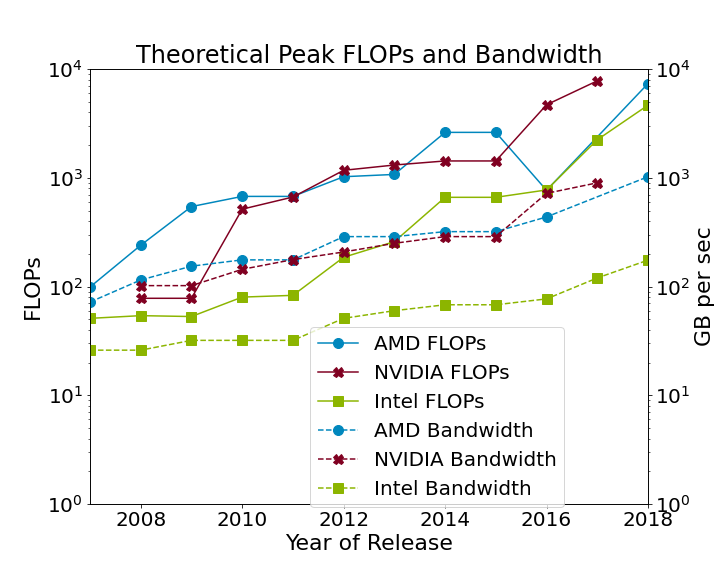
\includegraphics[width=.99\linewidth]{img/peakFlopsAndBandwidth}
\caption{Peak FLOPs and Bandwidth}
\end{subfigure}
\begin{subfigure}{.49\textwidth}
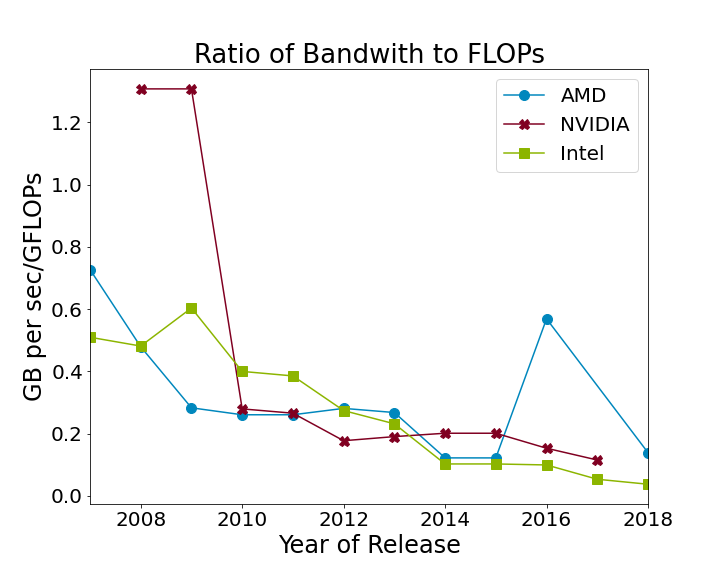
\includegraphics[width=.99\linewidth]{img/peakRatio}
\caption{Ratio Bandwidth to FLOPs}
\end{subfigure}
\caption{HPC System Balance}
\label{fig:peakratio}
\end{figure}

Using data from \cite{kruppcomparison}, we can see in Figure \ref{fig:peakratio} that AMD, NVIDIA, and Intel top of the line hardware has demonstrated a steady decrease in system balance, the ratio of maximum memory bandwidth to FLOPs, over the last 13 years.
HPC applications need to be careful to control the memory bandwidth required for their codes to better realize the FLOPs capabilities of HPC hardware.
High-order matrix-free finite element operators provide one way to reduce memory bandwidth requirements for HPC application codes.
